\let\negmedspace\undefined
\let\negthickspace\undefined
\documentclass[journal]{IEEEtran}
\usepackage[a5paper, margin=10mm, onecolumn]{geometry}
%\usepackage{lmodern} % Ensure lmodern is loaded for pdflatex
\usepackage{tfrupee} % Include tfrupee package

\setlength{\headheight}{1cm} % Set the height of the header box
\setlength{\headsep}{0mm}  % Set the distance between the header box and the top of the text

\usepackage{gvv-book}
\usepackage{gvv}
\usepackage{cite}
\usepackage{amsmath,amssymb,amsfonts,amsthm}
\usepackage{algorithmic}
\usepackage{graphicx}
\usepackage{textcomp}
\usepackage{xcolor}
\usepackage{txfonts}
\usepackage{listings}
\usepackage{enumitem}
\usepackage{mathtools}
\usepackage{gensymb}
\usepackage{comment}
\usepackage[breaklinks=true]{hyperref}
\usepackage{tkz-euclide} 
\usepackage{listings}
% \usepackage{gvv}                                        
\def\inputGnumericTable{}                                 
\usepackage[latin1]{inputenc}                                
\usepackage{color}                                            
\usepackage{array}                                            
\usepackage{longtable}                                       
\usepackage{calc}                                             
\usepackage{multirow}                                         
\usepackage{hhline}                                           
\usepackage{ifthen}                                           
\usepackage{lscape}
\begin{document}

\bibliographystyle{IEEEtran}
\vspace{3cm}

\title{11.16.3.17.1}
\author{EE24BTECH11015 - Dhawal}

% \maketitle
% \newpage
% \bigskip
{\let\newpage\relax\maketitle}

\renewcommand{\thefigure}{\theenumi}
\renewcommand{\thetable}{\theenumi}
\setlength{\intextsep}{10pt} % Space between text and floats

\textbf{Question:}\\
$P\brak{A}=0.42.$ Find $P\brak{A^c}$\\
	
	\textbf{Theoritical Solution:}
	\begin{align}
		P\brak{A^c}&=1-P\brak{A}\\
        P\brak{A^c}&=0.58
	\end{align}\\
	\textbf{Computational Solution:}\\
	Using Bernoulli Distribution.
    \begin{align}
        A\implies 1  &&  A^c \implies 0
    \end{align}

    The PMF represents the probability of each outcome in the sample space $S$ . For this
\begin{align*}
    S = \sbrak{0, 1},
\end{align*}

the PMF is given as:
\begin{align}
P(X = n) = 
\begin{cases} 
0.42 & n=1, \\ 
0.58 & n=0, \\ 
0 & n \notin S.
\end{cases}
\end{align}

\subsection*{Simulation Process}
Using random function $1000$ times obtain $0$ or $1$, where $P\brak{1}=0.42$ 
\begin{align}
    P\brak{A}=\frac{\text{Number of 1}}{1000}\\
        P\brak{A^c}=\frac{\text{Number of 0}}{1000}
\end{align}

	\subsection*{Final Solution}
	We get,
    \begin{align}
        P\brak{A}=0.4238 \\
        P\brak{A^c}=0.5762
    \end{align}

\begin{figure}[h]
    \centering
    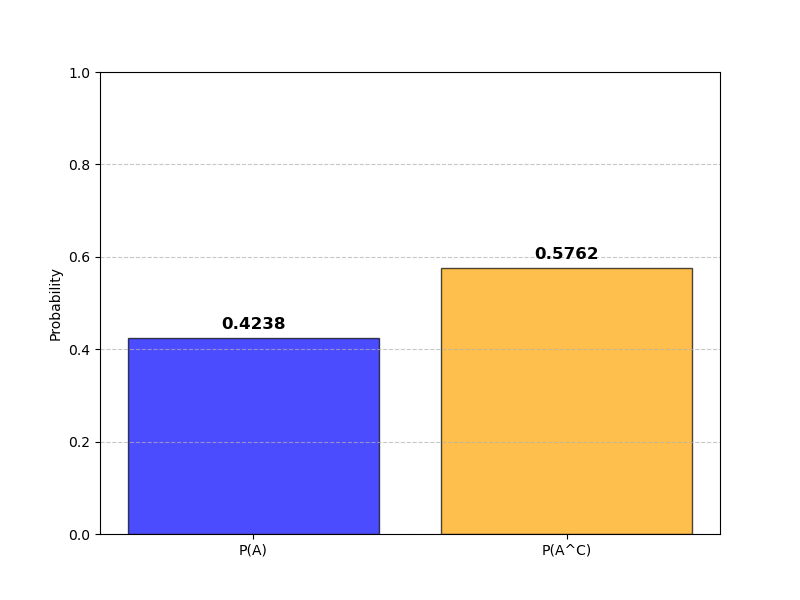
\includegraphics[width=\columnwidth]{figs/Figure_1.png}
    \label{fig:Plot}
    \end{figure}


\end{document}
